
\documentclass[11pt]{article}

\usepackage{ifpdf}
\usepackage{listings}
\lstset{
  frame=none,
  xleftmargin=2pt,
  belowcaptionskip=\bigskipamount,
  captionpos=b,
  escapeinside={*'}{'*},
  language=haskell,
  tabsize=2,
  emphstyle={\bf},
  commentstyle=\it,
  stringstyle=\mdseries\rmfamily,
  keywordstyle=\bfseries\rmfamily,
  columns=flexible,
  basicstyle=\small\sffamily,
  morecomment=[l]\%,
}
\ifpdf 
    \usepackage[pdftex]{graphicx}   % to include graphics
    \pdfcompresslevel=9 
    \usepackage[pdftex,     % sets up hyperref to use pdftex driver
            plainpages=false,   % allows page i and 1 to exist in the same document
            breaklinks=true,    % link texts can be broken at the end of line
            colorlinks=true,
            pdftitle=My Document
            pdfauthor=My Good Self
           ]{hyperref} 
    \usepackage{thumbpdf}
\else 
    \usepackage{graphicx}       % to include graphics
    \usepackage{hyperref}       % to simplify the use of \href
\fi 
\graphicspath{ {images/} }

\title{Report}
\author{Giovanni Garufi}
\date{}

\begin{document}
\maketitle

\section{Introduction}
Version control systems (VCS) have been steadily becoming an ubiquitous and central 
tool in programming. Many big projects, with hundreds of collaborators, 
fundamentally rely on these kind of tools to allow collaborators to interact 
with one another and to keep a structured log of the units of change. 
At the heart of most modern VCS is the unix diff utility. This tool computes a 
line-by-line difference between two files of text, determinig the smallest set 
of insertions or deletions of lines that transform one file into the other, this is called an edit script. 
Edit scripts are used when two collaborators have modified the same source file in independent 
ways and the VCS wants to reconcile the two independent changes into a single 
one. This operation is clearly not always possible: if two collaborators have 
modified the same line , in which case the two resulting edit scripts will 
``overlap'', it is not clear which one of the two modifications should be 
picked.  \\
In general, some conflicts will always require a manual intervention: when two 
people change the same thing in two different ways there is no general way of 
deciding which one will be the one we want to pick; however the diff tool makes 
a big assumption in considering lines to be the basic units in which change is 
observable.  \\
According to diff, two unrelated changes on the same line would still give rise to a 
conflict that requires manual intervention. 
The main idea of this reasearch is to design an alternative to diff which offers a 
finer grained control over the units of change, approaches similar to this one have already been explored in 
\cite{semantics-VC}, \cite{structure-aware-VC} and \cite{vassena}. In particular, in the context of 
programming languages we already have abstract syntax trees (AST) that encode 
the semantical structure of a program. By attempting to extend diff on the AST 
we gain both more control over the units of change, as a single line will 
usually contain multiple AST nodes and we gain information about the structure, encoded in the types which 
we can use to create transformation that operate on this structure in a principled way. 
The drawback of this approach is that it moves the problem from the ``flat'' 
world of strings to the ``layered'' world of trees, and the problem of computing an edit script between them suddendly
becomes much more computationally expensive. 
\\\\
The following section is an introduction to dependent types in haskell as they will be crucial in encoding 
the structure we want to express in our data types and their transformations. 
Following dependent types we will need to introduce sums of products: these give us a general way to view 
types and will allow us to define an algorithm that is independent of the representation of the AST for the language 
we are treating.
In the remainder of the proposal we will show a full Haskell implementation of the algorithm presented in 
\cite{type-directed-diff}, which is coded in Agda in the original paper. Finally we will explore some of the possible 
future directions that can be explored with this framework both in terms of 
gathering concrete evidence and in further research.

\section{Dependent types in
Haskell}\label{dependent-types-in-haskell}

With time, Haskell's type system has kept evolving from its humble
Hindley-Miller origins and through the use of different language extensions it has gained the ability 
to express more complex types. In particular, many efforts have gone to add support for dependently
typed programming in the latest years.

One major stepping stone in this direction is the DataKinds (\cite{datakinds}) extension which duplicates an ordinary data type, such as

\begin{lstlisting}[language=haskell]
data Nat = Z | S Nat
\end{lstlisting}

at the kind level, this means that from this declaration we automatically get two new types, namely \texttt{Z} of kind \texttt{Nat}
and \texttt{S} of kind \texttt{Nat\ -\textgreater{}\ Nat}.

We can use the \texttt{Nat} kind to index generalized algebraic data
types (GADTs) in a way that allows us to create an analogue of a
dependent type. In the case of \texttt{Nat}, we can use it to define a
GADT for vectors of a given length.

\begin{lstlisting}[language=haskell]
data Vec :: * -> Nat -> * where
  Vn ::                   Vec x Z
  Vc :: x -> Vec x n -> Vec x (S n)
\end{lstlisting}

Such a vector is either the empty vector, which is indexed by
\texttt{Z}, or a vector which is built by concatenating an element of
type \texttt{x} to a vector of \texttt{xs} of length \texttt{n},
yielding a vector of \texttt{xs} of length \texttt{S\ n}.

This allows us to define principled analogues of some functions which
operate on lists. The infamous \texttt{head} function will
crash our program when passed an empty list; equipped with these \texttt{Vec}, we can rule this
out by construction. 

This is how we can define a \texttt{head} function on vectors.

\begin{lstlisting}[language=haskell]
head :: Vec x (S n) -> x
head (Vc h t) = h
\end{lstlisting}

Informally, we are saying that the \texttt{head} function takes as
argument a vector with length strictly greater than 0. In this way, if we
try to pass an empty vector to \texttt{head} we will get a compile time
error instead of the usual runtime one.

Another extension which plays a crucial role in dependent types is
\texttt{TypeFamilies}: informally it allows us to write functions which operate on types, 
we will use this to define concatenation between \texttt{Vec}s.

The following type family can be seen as a function that takes two types
of kind \texttt{Nat} and returns another type of kind \texttt{Nat}
representing the result of adding those two types.

\begin{lstlisting}[language=haskell]
type family (m :: Nat) :+ (n :: Nat) :: Nat where
  Z      :+ n = n
  (S m) :+ n = S (m :+ n)
\end{lstlisting}

Equipped with this type family we can now define concatenation between
vectors.

\begin{lstlisting}[language=haskell]
vappend :: Vec x n -> Vec x m -> Vec x (n :+ m)
vappend Vn          ys = ys
vappend (x `Vc` xs) ys = x `Vc` (vappend xs ys)
\end{lstlisting}

One interesting thing to note is that up to this point, we never use the
\texttt{Nat} part of a vector at runtime. That information is only used
at compile time to check that everything ``lines up'' the way it should
be, but could actually be erased at runtime.

Suppose we want to write a \texttt{split} function, this function takes
an \texttt{n} of kind \texttt{Nat}, a vector of length \texttt{n\ :+\ m}
and splits it into a pair of vectors, with respectively \texttt{n} and
\texttt{m} elements.

The first problem we incur in is that we can not pass something of kind
\texttt{Nat} to our \texttt{split} function, infact the types \texttt{K} and \texttt{S} have no inhabitants, so we can
not construct any term of those types. Furthermore, we want to
express that this \texttt{n} of kind \texttt{Nat} that we pass as a
first argument, is the same \texttt{n} as in the vector length. The idea is to 
wrap this type into a singleton data type, giving us a dynamic container of the static 
information.

\begin{lstlisting}[language=haskell]
data SNat :: Nat -> * where
  SZ ::           SNat Z
  SN :: SNat n -> SNat (S n)
\end{lstlisting}

The name singleton comes from the fact that each type level value of
kind \texttt{Nat} (namely \texttt{Z} or \texttt{S} applied to another
type of kind \texttt{Nat}) has a single representative in the
\texttt{SNat} type.

The following figure gives a good representation of this process: the
DataKinds extensions promotes things of type \texttt{Nat} to things of
kind \texttt{Nat}. The singleton allows us to take one step back in this
ladder, and associates to every thing of kind \texttt{Nat} a term from
the singleton type \texttt{SNat}. The following picture, borrowed from \cite{singletons}, gives a good 
represenation of this process.

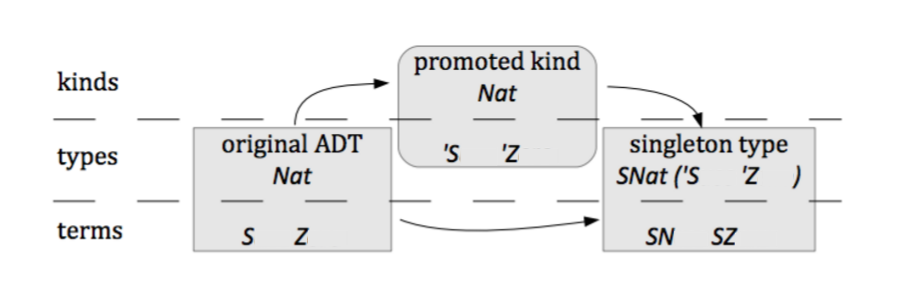
\includegraphics[width=\textwidth]{singleton.png}


We can think of the DataKinds extension as a way of embedding dynamic information into the static fragment of 
the language. Singletons, on the other hand, are a way to reflect this static information back to 
the dynamic level, and make runtime decisions based on the types we obtain.


Singletons solve the two problems outlined above: they have kind \texttt{*}
and it contains a \texttt{Nat} that we can later refer to in our
function definition. We can now define \texttt{split} as follows:

\begin{lstlisting}[language=haskell]
split :: SNat n -> Vec x (n :+ m) -> (Vec x n, Vec x m)
split SZ     xs          = (Vn, xs)
split (Sn n) (x `Vc` xs) = (x `Vc` ys, zs)
  where
    (ys, zs) = split n xs
\end{lstlisting}

With these three tricks up our sleeve: data kind promotion, type level
functions and singletons we can emulate some of the features that are
present in dependently typed languages such as Agda. These features allow us to 
emulate explicit dependent quantification; we can actually go even further in 
Haskell, \cite{hasochism} shows us how to emulate implicit types via type 
classes and ultimately shows how all kinds of quantification, modulo some boilerplate, are possible in 
Haskell.

\section{Sum of Products}

Another key idea that we will explore is related to the representation of 
generic datatypes. The basic idea is to view any term as the result of applying 
one constructor of the type the term inhabits to a list of arguments (which may also be other terms of the
same type). It is useful to think about the choice of constructor and the choice 
of arguments as two different levels. On the first level we 
make a choice about which constructor to pick, this corresponds to a sum
over all the constructors of the type. On the second level, we are choosing a certain number of arguments 
to feed to that constructor and this can be viewed as a list, or product, of 
those arguments. Clearly the products will depend on the choice of constructor, 
each of which possibly takes a different number of arguments of possibly 
different types. A constructor can also take no arguments, in which case we 
can simply use an empty list to represent that, but can also take an argument of 
the same type it is trying to construct (like the \texttt{S} constructor from the previous example). 
In this case, the recursive argument can itself be encoded as an \texttt{SOP} 
and the same encoding can be used all the way down to the leaves. 
Since every data type can be encoded as an \texttt{SOP}, we can write functions 
that act on this representation and regard them as generics. For every data type 
we can first convert it to the \texttt{SOP} representation and then pass it to 
the desired function, since the \texttt{SOP} representation can be easily 
seen to be isomorphic to the original type, we can eventually reconstruct the 
desired term once we are done acting on the representation. This encoding is 
presented in \cite{true-sop} and represents one of the different ways to 
approach generic programming in Haskell

\section{Type-directed diff}\label{type-directed-diff}

The approach in \cite{type-directed-diff} takes advantage of the structure 
encoded in types to define a generic type-directed diff algorithm between
typed trees. The inspiration comes from the diff utility present in
Unix which is at the heart of the current methodologies employed by VCS
to attempt to compute a patch between two different versions of the same
file. The limitations of the diff algorithm, as it currently stands, is
that it does not employ any structural information between the data it
is trying to merge. Files are parsed on a line by line basis and, as
the authors of \cite{type-directed-diff} show, this is somewhat resilient to vertical changes in the
source code but completely breaks down when dealing with horizontal
changes, which constitute a heavy chunk of the changes that are usually
made to code.

The underlying idea to the approach presented in the article is to employ
the generic SoP view presented in the preceding section to define a
generic way to view datatypes. Once that is settled, we obtain a view of
any well defined program as a structured tree of data, where each object
we inspect can be represented as a choice of a certain constructor,
among the available ones, and a choice of arguments to that constructor.
This process is equivalent to parsing the source language into an AST,
an interesting consideration to make is that the choice of AST for
diffing purposes might be very different from the representation that
would be chosen for a compiler of the language. While these two
structures should be ``somewhat isomorphic'', the amount of domain
specific knowledge that should be represented in the AST is certainly
not necessarily the same, one of the goals of this work is to explore
this boundary and the choice of what kind of information is beneficial
for calculating a patch between these two structures.

We will briefly sketch the process outlined in \cite{type-directed-diff}, it 
will be covered in more detail in the following section about the 
implementation.
\ 
In the process of transforming one tree into another we need to keep track of three different things: 
changes on the constructor level, changes on the product (the arguments to the constructors) 
level, and finally changes on each element of the product (we will call these 
atoms).
\subsection{Spine}\label{spine}

Calculating a spine for two trees corresponds to calculating the
longest common prefix between two strings. Recall that the two trees
\emph{x} and \emph{y} are viewed as SoP, in this sense calculating the
spine between \emph{x} and \emph{y} corresponds to capturing the common
coproduct structure between them. In general, we have three cases to
consider. 
\begin{itemize}
  \item x = y 
  \item x and y have the same constructor but not all the
subtrees are equal  
  \item x and y have different constructors
\end{itemize}
 This gives rise
to three different constructors for the Spine datatype, each
corresponding to one of the cases described above.

The spine tracks only relationships between the sum types but information
about changes on the product level must be carried along too. In the
case that the constructor has remained the same, we can group up the
pairs of arguments and proceed from there; however, in the case the
external constructor has changed, there is no obvious way of pairing up
the arguments (they might be completely in different numbers and types), this 
motivates the following definition of alignments.

\subsection{Alignment}\label{alignment}

As mentioned in the previous paragraph, the spine takes care of matching
the constructors of two trees, beyond that we still need to define a way
to continue diffing the products of data stored in the constructors.
Recall that this alignment has to work between two heterogeneous lists
corresponding to the fields associated with two distinct constructors.
The approach presented below is inspired by the existing algorithms
based on the edit distance between two strings. The problem of finding
an alignment of two lists of constructor fields can be viewed as the
problem of finding an edit script between these two. An edit script is
simply a sequence of operations which describe how to change the source
list into the destination. In computing an edit script we simply
traverse the lists, from left to right considering one element from each
list. At each step we are presented with three choices:

\begin{itemize}
\item
  We can match the two elements (Amod) of the list and continue
  recursively aligning the rest
\item
  We can insert the destination element before the current element in
  the source list (Ains) and recursively compute an alignment between
  whatever we have in the source list and the tail of the destination.
\item
  We can delete the element from the source list (Adel) and recursively
  compute the alignment between the rest of the source and the
  destination.
\end{itemize}

This approach is inspired by the way an edit script between two strings
can be computed, there is one major difference though: while in the
string case we can assume deletions and insertions to be somewhat
equivalent in cost (thus we can safely try to maximize one of the two)
in our case, where the elements we are inserting or deleting are
arbitrary big subtrees it is not obvious if we should try and maximize
insertions or deletions.

The solution to this problem is simple at this step: we simply enumerate
all possible alignments, avoiding to skew the algorithm into preferring
insertions over deletions or viceversa.

\subsection{Atoms}\label{atoms}

Having figured out all the alignments between two lists of constructor
fields we still have to decide what to do in the case where we match two
elements. Here we need to make a distinction between the possibly
recursive fields and the constant ones. In the case of constant fields
like \texttt{Int}s or \texttt{String}s, a transformation between two
values of this type is simply a pair recording the source value and the
destination value. In the case of a possibly recursive datatype we are
essentially left with the problem we started from: transforming a value
of a datatype into another. To do so, we simply start all over again,
recursively computing a spine and an alignment between constructor
fields.

\section{Implementation}\label{implementation}

The AST defined in the Parser module represents the parse result of
clojure source code. To set up the stage for the rest of the algorithm
we must start building up our universe from the AST, this process is
completely mechanical and could be automated via template haskell.

\subsection{Setting up the universe}\label{setting-up-the-universe}

An AST consists of a family of datatypes, with a main one which
represents the outer structure of the language, and a number of other
possibly mutually recursive datatypes appearing as arguments to the
constructors of the main datatype. This is a simple example of such a
family

\begin{lstlisting}[language=haskell]
data SExpr = List SExprList | Operation SExpr SExpr | Value Int
  deriving (Eq, Show)

data SExprList = SNil | SCons SExpr SExprList
  deriving (Eq, Show)
\end{lstlisting}

For each type that appears as an argument to a constructor in our family
of datatypes, we will construct an atom, representing that type.
Following the example above, we will define

\begin{lstlisting}[language=haskell]
data U = KInt | KSExpr | KSExprList
\end{lstlisting}

We will also need to associate with each atom a singleton, this will
allow us to relate the atoms back to the constructors in the original
family.

\begin{lstlisting}[language=haskell]
data Usingl :: U -> * where
  Uint    :: Int       -> Usingl KInt
  Usexpr  :: SExpr     -> Usingl KSExpr
  UsexprL :: SExprList -> Usingl KSExprList
\end{lstlisting}

Now, we can group all the constructors appearing in our original family
of datatypes under the \texttt{Constr} type, in a similar way that we
did for the atoms. To makes things easier to follow we prepend to the name of each
constructor a tag representing which family the constructor came from.

In this case \texttt{C1} is \texttt{SExpr} and \texttt{C2} is
\texttt{SExprList}.

\begin{lstlisting}[language=haskell]
data Constr =
    C1List
  | C1Operation
  | C1Value
  | C2SNil
  | C2SCons
\end{lstlisting}

Now we just need a way to relate constructors to the correct datatype in
the family. To achieve this, we define the \texttt{ConstrFor} datatype,
which can be viewed as a proof that a certain constructor builds element
of a certain family.

\begin{lstlisting}[language=haskell]
data ConstrFor :: U -> Constr -> * where
  C1ListProof      :: ConstrFor KSExpr C1List
  C1OperationProof :: ConstrFor KSExpr C1Operation
  C1ValueProof     :: ConstrFor KSExpr C1Value
  C2SNilProof      :: ConstrFor KSExprList C2SNil
  C2SConsProof     :: ConstrFor KSExprList C2SCons
\end{lstlisting}

Finally we must encode one last bit of information: the ``shape'' of
each constructor. To do so, we can use a closed type family which can be
viewed as a function on types. This function takes a \texttt{Constr} and
returns a list of atoms representing the arguments the constructor
accepts.

\begin{lstlisting}[language=haskell]
type family TypeOf (c :: Constr) :: [U] where
  TypeOf C1List           = '[KSExprList]
  TypeOf C1Operation = '[KSExpr, KSExpr]
  TypeOf C1Value       = '[KInt]
  TypeOf C2SNil         = '[]
  TypeOf C2SCons     = '[KSExpr, KSExprList]
\end{lstlisting}

Since \texttt{TypeOf} return something of kind \texttt{{[}U{]}} we will
define another GADT named \texttt{All}, that maps a type constructor
\texttt{k\ -\textgreater{}\ *} over an argument of kind \texttt{{[}k{]}}
giving us something of kind \texttt{*} to quantify over a list of types.

The definition for \texttt{All} is straightforward:

\begin{lstlisting}[language=haskell]
data All (k -> *) :: [k] -> * where
  An ::                    All p '[]
  Ac :: p x -> All p xs -> All p (x ': xs)
\end{lstlisting}

With this setup we can finally construct the \texttt{View} datatype,
this loosely corresponds to a generic view as sum of products of a
datatype, and simply deconstructs each term of a type into a constructor
and a list of arguments applied to that constructor

\begin{lstlisting}[language=haskell]
data View u where
 Tag :: ConstrFor u c -> All Usingl (TypeOf c) -> View u
\end{lstlisting}

\subsection{The actual puzzle}\label{the-actual-puzzle}

We are now going to show how to define data types to represent spines, 
alignments and atoms. We will also need a way to tie the recursive knot 
mentioned in the previous section about atoms: essentially we need to define a way to 
differentiate between constant and recursive atoms and treat them accordingly.

\paragraph{Spine}\label{spine-1}

We will start from the spine: as mentioned in the previous section, a
spine represents the common structure between two elements of a type. In
constructing it we must account for three different cases: if the two
elements are the same, the spine is trivially a copy, if the top level
constructors match, the spine consists of this information and a way to
transform the paris of constructor fields and lastly if two constructors
don't match, the spine must record this and also contain a way to
transform the list of source fields into the list of destination fields.
This can be captured in Haskell by the following GADT:

\begin{lstlisting}[language=haskell]
data Spine (at :: U -> *)(al :: [U] -> [U] -> *) :: U -> * where
  Scp  :: Spine at al u
  Scns :: ConstrFor u s -> All at (TypeOf s) -> Spine at al u
  Schg :: ConstrFor u s -> ConstrFor u r
       -> al (TypeOf s) (TypeOf r)
       -> Spine at al u
\end{lstlisting}

The third parameter of the spine (the \texttt{U}) represents the
underlying type for which we are trying to compute the transformation,
the other two parameters, \texttt{al} and \texttt{at} are respectively: a
function between products that describes what to do with the different
constructor fields and a predicate between atoms which describes what to
do with the paired fields in case we have the same constructor. The
\texttt{Scp} constructor corresponds to the first case, in which we need
to record no additional information other than the fact that the two
elements are equal. The \texttt{Scns} constructor corresponds to the
second case: the first argument records the common constructor for the
two elements and the second represents the list of paired atoms to which
we apply the \texttt{at} predicate. The \texttt{Schg} constructor
represents a change of constructor: the first two arguments record the
source and destination constructors, and the third argument is the
\texttt{al} function applied to the constructor fields of the source and
destination constructor respectively.

\paragraph{Alignments}\label{alignments}

Now we need to define a type representing alignments, similarly to the
spine, the alignment is parametrized by a predicate \texttt{at} which
describes how to treat the underlying atoms. The specification outlined
above is captured by the following GADT

\begin{lstlisting}[language=haskell]
data Al (at :: U -> *) :: [U] -> [U] -> * where
  A0   :: Al at '[] '[]
  Ains :: Usingl u -> Al at xs ys -> Al at xs (u ': ys)
  Adel :: Usingl u -> Al at xs ys -> Al at (u ': xs) ys
  Amod :: at u -> Al at xs ys -> Al at (u ': xs) (u ': ys)
\end{lstlisting}

\texttt{A0} represents the empty alignment, \texttt{Ains} and \texttt{Adel} take as first argument
a singleton representing a runtime instance of the type u and, together
with an alignment for the rest of the list, give us the alignment with
an insertion (resp. deletion) as explained in the section above. In the
\texttt{Amod} case: the first argument is the predicate on the underlying atom
and the other, like for insertions and deletions, is simply an alignment for the tail of the 
list.

\paragraph{Atoms}\label{atoms}

Given to atoms x and y we have two cases: they can either be both recursive elements 
of the language: in which case we have to proceed recursively computing a diff 
between them, or, they might both be constant values: in that case we can simply 
build a pair out of them relating the source and destination value.

To represent these pairs we can introduce a helper \texttt{Contract} datatype which 
lifts f over a pair of xs.

\begin{lstlisting}[language=haskell]
  newtype Contract (f :: k -> *) (x :: k) = Contract { unContract :: (f x , f x) }
\end{lstlisting}

To distinguish between recursive and non recursive elements of the language we 
define a typeclass with no additional methods, and add instances of this typeclass only for the recursive atoms.

Once again, borrowing the language definition in the previous section, we will have the following 
class and instances defined
\begin{lstlisting}[language=haskell]
class IsRecEl (u :: U) where
instance IsRecEl KSExpr where
instance IsRecEl KSExprList where
\end{lstlisting}

With this we can define the following datatype to represent diffs between atoms of our language.
\begin{lstlisting}[language=haskell]
data At (recP :: U -> *) :: U -> * where
  Ai :: (IsRecEl u) => recP u -> At recP u
  As :: Contract Usingl u -> At recP u
\end{lstlisting}
\paragraph{Recursive alignments}\label{recursive alignments}

Finally we have to define a datatype to represent changes over our recursive 
elements. We mirror the treatment of alignement for list of atoms but instead, on this level, we 
match, insert or delete constructors instead of atoms. 
A match of constructors will be represented as a spine while insertions and 
deletions will record the constructor being inserted (resp. deleted) and a 
\texttt{Ctx} which records which fields are associated to that constructor.
\texttt{Ctx}s are inspired by zippers: they can be thought as a representation 
of a  type with a hole somewhere; the hole representse th place where we 
plug in the rest of the tree to continue the computation.
\begin{lstlisting}[language=haskell]
data Almu :: U -> U -> * where
  Alspn :: Spine (At Almu) (Al (At Almu)) u -> Almu u u
  Alins :: ConstrFor v s -> Ctx (Almu u) (TypeOf s) -> Almu u v
  Aldel :: ConstrFor u s -> Ctx (Almu v) (TypeOf s) -> Almu u v
\end{lstlisting}
\
\paragraph{Putting everything together}\label{putting everything together}

With these types it is easy to write a function that computes the diff between 
two trees.
We can start writing this function from the ``bottom up'' 
with the definition of a diff between two atoms. The function should have the 
following signature
\begin{lstlisting}
  diffAt ::  (forall r . IsRecEl r => Usingl r -> Usingl r -> [rec r])
            -> Usingl a -> Usingl a -> [At rec a]
\end{lstlisting}
This function is parametrized by a function that describes the treatment for 
recursive atoms. By inspecting the first singleton we learn wether the atom is 
recursive or not; if that is the case, the function that deals with the 
recursive elements can be used to build the corresponding \texttt{At}. In the 
other case, when the element is non recursive, we can simply pair up the two 
constant atoms with a \texttt{Contract} and build the non recursive \texttt{At}.

We can then proceed by implementing the function that computes all the spines 
between recursive elements.
\begin{lstlisting}
 diffS :: IsRecEl a => (forall r . IsRecEl r => Usingl r -> Usingl r -> [rec r])
        -> Usingl a -> Usingl a -> [Spine (At rec) (Al (At rec)) a]
\end{lstlisting}
Which lifts the parameter it takes, a function to handle the 
recursive elements of our language, over the predicate parameters to the spine that results 
from the two singletons.

We finally have to define a function that computes the diff in terms of 
\texttt{Almu}s. This will call \texttt{diffS} in case of two matching constructors from which we can compute
the spine wrapping that with the corresponding \texttt{Alspn} constructor. In the other cases it will 
attempt the inesertion (resp. deletion) at the constructor level by recording the constructor being inserted
(deleted) and producing a \texttt{Ctx} which describes where the original tree is attached in respect to
the added (deleted) constructor.
This function will have the following signature

\begin{lstlisting}
  diffAlmu :: (IsRecEl u, IsRecEl v) => Usingl u -> Usingl v -> [Almu u v]
\end{lstlisting}

As is the case for the alignment between products, here we will simply proceed 
by enumerating all possible recursive alignments, attempting at each level 
the alignment of spines, insertions and deletions.
One shortcoming with this approach, lies in the great combinatorial 
explosion of possibilities that arises in computing the alignments for 
constructors and products. The following paragraph will describe an optimization 
we can employ to prune the number of possible alignments. This optimization 
will allow the program to run in an acceptable time in real world scenarios, however 
we are still at least an order of magnitude slower than diff3, this points to 
the necessity of further and more aggressive optimizations that may be explored 
in future work.

\paragraph{Optimization}\label{optimizations}

Given the \texttt{Al} and \texttt{Almu} type defined in the previous paragraphs we are still left with the problem
to computing these two level of alignments. Since we don't know apriori which alignment
is more efficient we will non-deterministically compute all the possible ones. The number of all possible alignments  
can grow very quickly; to make things worse: we are dealing with alignments of arbitrarily large subtrees, which prevents
us from optimizing towards insertions or deletions. It is easy to see
that in some cases, prioritizing deletions can be more profitable and in
other it may be better to do the opposite; this uncertainty stems from
the fact that at the time we are calculating the alignment we have no
information about the size of the subtrees we are considering.

There is one optimization we can introduce, despite this limitation: in
the case where we can match a pair of elements then we can avoid
computing an insertion followed by a deletion (resp. a deletion followed
by an insertion) since the case in which we match is at least ``as
good'' as the case in which we perform the two different operations in
sequence, regardless of the actual cost we are assigning to each
operation.

To implement this we must add a parameter that tracks the operation that
was taken at the previous step, we will call this the \texttt{Phase}. We
can define an \texttt{alignOpt} function with the same signature as
\texttt{align} but parametrized with the \texttt{Phase}. The optimized
version will simply avoid performing an insertion if the last step was a
deletion and vice versa. 
After every succesfull match, we will call \texttt{alignOpt} to enumerate the alternatives for both insertions and
deletions. In the case in which we could not match, we don't 
want to attempt both a deletion followed by an insertion and insertion followed by a deletion, as the 
ordering between the two does not really matter. To resolve this we will simply 
decide that we will only try deletions followed by insertions, and not the other 
way around.

The optimization con be used on the two different levels; the same idea is used to prune the search space 
for both the alignment between the list of atoms and the recursive alignment between constructors.


\subsection{Evaluation process}

Having developed a general framework to compute patches between typed trees the 
goal is to explore its performance in the context of a real programming 
language.
To test this, we developed a parser for Clojure, the implementation of this parser can be somewhat 
different to one designed to interpret and run Clojure code. While it may 
be fruitful to encode as much domain specific knowledge into the parser, thus 
enabling possible further optimizations; it is also clear that the parser should 
capture as much syntactical information as possible, in order to produce code 
that strives to respect any syntactical convention embraced by the authors.

In order to test the framework in a real world context we need to find some suitable data. To aquire this 
we explored all the Clojure repositories on Github and extraced the ones with the best combination of 
stars and collaborators. A high number of collaborators will possibly imply a higher chance for conflicts in
the source tree, the high number of stars is a good indicator of the quality of 
the Clojure code and hopefully provides a selection of repository from different 
domains.

What we need is a way to identify merge points in a projects history, we also 
want to know how diff3 performed in those merges, in essence: we want to find all 
merge points and record if the merge was performed automatically or a conflit 
had to be manually fixed.

For each file where a conflict may arise we want to find a common ancestor 
between the branches and calculate two sets of patches, transforming this file 
into the two versions that are currently present at the top of their respective 
tree. 

We aim to define a notion of disjointness between patches which 
encodes the fact that the two patches don't apply conflicting transformations 
between each other. We expect disjoint patches to commute in the order they can 
be applied, experimentation could yield a counterexample to this conjecture but 
on the other hand could also provide good insight into the exact notion of 
disjointness that is needed between patches.

Finally we want to explore with different heuristics to score patches, this will 
have both the advantage of allowing us to greedily prune the search space for 
alignments (both recursive and non) and possibly also correlate with 
disjointness, in the sense that on optimal patch should strive to be minimal, 
and, as such, as disjoint as possible from every other patch with the same source.

\section{Future Work}\label{future work}
The optimization described in the previous section is probably still not suited 
for large real world applications. Even with the optimization the framework can only handle relatively small 
non-pathological inputs (in the order of 10-15 lines), clearly this is still not good enough to perform experiments
on real world data. One possible direction in which to focus future work is to explore the 
possibility of using the standard unix \texttt{diff3} algorithm as an oracle to prune the 
alignment trees that are being generated. 
The idea is that instead of enumerating all possible alignments between two 
trees, we can check and see how \texttt{diff3} treats the sequence of lines in which that 
tree resides in the source. This can allow us to prune the search space based on 
the information we can derive from \texttt{diff3} and may be able to speed up 
the computation to handle larger inputs.

Another subject to explore is to extend what was done up to this point to define 
a precise notion of a merge between two patches which is the main motiviation of the 
research. This is tightly related to disjointness; informally disjoint 
patches operate on different parts of the origin file and for that reason should 
be mergeable into a single patch that incorporates both changes. 

The resulting patch objects that are generated are very complex and contain deeply nested information which is 
not easy to pick up at a glance. 
Existing diff tools often prepend a  plus or minus sign at the beginning of a line to signal it being deleted or 
inserted and have custom notation for conflicts. In our case the problem is 
complicated by the fact that information can not only be displayed along the 
different lines but also inside of them. 
It would be useful to have a representation of these patches which conveys the information 
they represent in an easy to digest way, this representation could as well be 
interactive (possibly in HTML) in order to facilitate the navigation through the 
different levels of the patch.


\begin{thebibliography}{9}
  

\bibitem{hasochism}
  Lindley, Sam, and Conor McBride. "Hasochism: the pleasure and pain of dependently typed Haskell programming." ACM SIGPLAN Notices 48.12 (2014): 81-92.

\bibitem{singletons}
  Eisenberg, Richard A., and Stephanie Weirich. "Dependently typed programming with singletons." ACM SIGPLAN Notices 47.12 (2013): 117-130.
\bibitem{datakinds}
  Yorgey, Brent A., et al. "Giving Haskell a promotion." Proceedings of the 8th ACM SIGPLAN workshop on Types in language design and implementation. ACM, 2012.
  
 \bibitem{structure-aware-VC}
   Miraldo, Victor Cacciari, and Wouter Swierstra. "Structure-aware version control: A generic approach using Agda." (2017).

\bibitem{semantics-VC}
  Swierstra, Wouter, and Andres Löh. "The semantics of version control." Proceedings of the 2014 ACM International Symposium on New Ideas, New Paradigms, and Reflections on Programming & Software. ACM, 2014.
  
\bibitem{vassena}
  Vassena, Marco. "Generic Diff3 for algebraic datatypes." Proceedings of the 1st International Workshop on Type-Driven Development. ACM, 2016.

\bibitem{type-directed-diff}
  ???
  
\bibitem{true-sop}
  de Vries, Edsko, and Andres Löh. "True sums of products." Proceedings of the 10th ACM SIGPLAN workshop on Generic programming. ACM, 2014.
 \end{thebibliography}
\end{document}  



